% This is "sig-alternate.tex" V1.9 April 2009
% This file should be compiled with V2.4 of "sig-alternate.cls" April 2009
%
% This example file demonstrates the use of the 'sig-alternate.cls'
% V2.4 LaTeX2e document class file. It is for those submitting
% articles to ACM Conference Proceedings WHO DO NOT WISH TO
% STRICTLY ADHERE TO THE SIGS (PUBS-BOARD-ENDORSED) STYLE.
% The 'sig-alternate.cls' file will produce a similar-looking,
% albeit, 'tighter' paper resulting in, invariably, fewer pages.
%
% ----------------------------------------------------------------------------------------------------------------
% This .tex file (and associated .cls V2.4) produces:
%       1) The Permission Statement
%       2) The Conference (location) Info information
%       3) The Copyright Line with ACM data
%       4) NO page numbers
%
% as against the acm_proc_article-sp.cls file which
% DOES NOT produce 1) thru' 3) above.
%
% Using 'sig-alternate.cls' you have control, however, from within
% the source .tex file, over both the CopyrightYear
% (defaulted to 200X) and the ACM Copyright Data
% (defaulted to X-XXXXX-XX-X/XX/XX).
% e.g.
% \CopyrightYear{2007} will cause 2007 to appear in the copyright line.
% \crdata{0-12345-67-8/90/12} will cause 0-12345-67-8/90/12 to appear in the copyright line.
%
% ---------------------------------------------------------------------------------------------------------------
% This .tex source is an example which *does* use
% the .bib file (from which the .bbl file % is produced).
% REMEMBER HOWEVER: After having produced the .bbl file,
% and prior to final submission, you *NEED* to 'insert'
% your .bbl file into your source .tex file so as to provide
% ONE 'self-contained' source file.
%
% ================= IF YOU HAVE QUESTIONS =======================
% Questions regarding the SIGS styles, SIGS policies and
% procedures, Conferences etc. should be sent to
% Adrienne Griscti (griscti@acm.org)
%
% Technical questions _only_ to
% Gerald Murray (murray@hq.acm.org)
% ===============================================================
%
% For tracking purposes - this is V1.9 - April 2009

\documentclass{sig-alternate}
\usepackage{pgf}
\usepackage{listings}
\usepackage{url}
\usepackage{subfigure}

\definecolor{darkgreen}{rgb}{0,0.7,0}
\definecolor{violet}{rgb}{0.5,0.0,0.5}

\newcommand{\up}{\vspace*{-1em}}
\newcommand{\upp}{\vspace*{-0.5em}}
\lstset{language=bash, numbers=left, numberstyle=\tiny\color{gray}, numbersep=3pt, escapeinside={\$}, basicstyle=\footnotesize\ttfamily, escapeinside={\%*}{*)}}

\newif\ifdraft
\drafttrue
%\draftfalse                                                                              
\ifdraft
\newcommand{\iannote}[1]{ {\textcolor{red}    { ***Ian:      #1 }}}
\newcommand{\katznote}[1]{ {\textcolor{blue}    { ***Dan:      #1 }}}
\newcommand{\zhaonote}[1]{{\textcolor{darkgreen}    { ***Zhao:      #1 }}}
\newcommand{\armnote}[1]{{\textcolor{violet}    { ***Tim:      #1 }}}
\newcommand{\note}[1]{ {\textcolor{red}    {\bf #1 }}}
\else
\newcommand{\iannote}[1]{}
%\newcommand{\iannote}[1]{}
\newcommand{\katznote}[1]{}
\newcommand{\zhaonote}[1]{}
\newcommand{\note}[1]{}
\fi

 \newenvironment{shortlist}{
        \vspace*{-0.5em}
  \begin{itemize}
  \setlength{\itemsep}{-0.1em}
}{
  \end{itemize}
        \vspace*{-0.5em}
}

\hyphenation{Map-Reduce}


\begin{document}
\title{Application Skeletons: Encapsulating MTC Application Task Computation and I/O}


%\subtitle{[Extended Abstract]
%\titlenote{A full version of this paper is available as
%\textit{Author's Guide to Preparing ACM SIG Proceedings Using
%\LaTeX$2_\epsilon$\ and BibTeX} at
%\texttt{www.acm.org/eaddress.htm}}}
%
% You need the command \numberofauthors to handle the 'placement
% and alignment' of the authors beneath the title.
%
% For aesthetic reasons, we recommend 'three authors at a time'
% i.e. three 'name/affiliation blocks' be placed beneath the title.
%
% NOTE: You are NOT restricted in how many 'rows' of
% "name/affiliations" may appear. We just ask that you restrict
% the number of 'columns' to three.
%
% Because of the available 'opening page real-estate'
% we ask you to refrain from putting more than six authors
% (two rows with three columns) beneath the article title.
% More than six makes the first-page appear very cluttered indeed.
%
% Use the \alignauthor commands to handle the names
% and affiliations for an 'aesthetic maximum' of six authors.
% Add names, affiliations, addresses for
% the seventh etc. author(s) as the argument for the
% \additionalauthors command.
% These 'additional authors' will be output/set for you
% without further effort on your part as the last section in
% the body of your article BEFORE References or any Appendices.

\numberofauthors{2} %  in this sample file, there are a *total*
% of EIGHT authors. SIX appear on the 'first-page' (for formatting
% reasons) and the remaining two appear in the \additionalauthors section.
%
\author{
% You can go ahead and credit any number of authors here,
% e.g. one 'row of three' or two rows (consisting of one row of three
% and a second row of one, two or three).
%
% The command \alignauthor (no curly braces needed) should
% precede each author name, affiliation/snail-mail address and
% e-mail address. Additionally, tag each line of
% affiliation/address with \affaddr, and tag the
% e-mail address with \email.
%
% 1st. author
\alignauthor
Zhao Zhang\\
       \affaddr{Department of Computer Science}\\
       \affaddr{University of Chicago}\\
       \email{zhaozhang@uchicago.edu}
% 2nd. author
\alignauthor
Daniel S. Katz\\
       \affaddr{Computation Institute}\\
       \affaddr{University of Chicago \& Argonne National Laboratory}\\
       \email{d.katz@ieee.org}
}
% There's nothing stopping you putting the seventh, eighth, etc.
% author on the opening page (as the 'third row') but we ask,
% for aesthetic reasons that you place these 'additional authors'
% in the \additional authors block, viz.
%\additionalauthors{Additional authors: John Smith (The Th{\o}rv{\"a}ld Group,
%email: {\texttt{jsmith@affiliation.org}}) and Julius P.~Kumquat
%(The Kumquat Consortium, email: {\texttt{jpkumquat@consortium.net}}).}
%\date{30 July 1999}
% Just remember to make sure that the TOTAL number of authors
% is the number that will appear on the first page PLUS the
% number that will appear in the \additionalauthors section.

\maketitle

\begin{abstract}
Computer scientists who work on tools and systems meant to
support or enable a variety of distributed computing applications want to
prove that the systems they design actually help those applications.
However, doing this by using the actual applications can be
difficult due to policy or technical issues when accessing and building the application
and necessary data sets.  
These issues led us to the idea of an Application Skeleton -- a simple yet powerful tool to build synthetic applications that represent
real applications, with runtime, I/O, and intertask communication close to those of
the real applications. This allows computer scientists to focus on the system they are
building; they can work with the simpler Skeleton applications and be sure that their
work will also be applicable to the real applications.
Skeletons currently can create easy-to-access, easy-to-build,
and easy-to-run bag-of-task, map-reduce,
and multi-stage workflow applications. In this initial work, we show that a Skeleton
version of the Montage application has a runtime 
difference of 2.6\% in total on 64 processors on a BG/P supercomputer. And six of
eight stages have an error within 5\%.

\end{abstract}

   \lstset{
     basicstyle=\ttfamily\scriptsize,
     breaklines=true
   }

\section{Introduction}
Computer scientists who build tools and systems (programming languages, runtime systems, file systems, workflow systems, etc.) 
to support distributed applications often have to work on real scientific applications to prove the effectiveness of
the system. However, accessing and building the real applications is time consuming or sometimes infeasible due to one
or more of the following reasons:
\begin{shortlist}
\item {} Some applications (source) are privately accessible
\item {} Some data is difficult to access 
\item {} Some applications use legacy code and are dependent on out-of-date libraries
\item {} Some applications are hard to understand because of the knowledge gap between the computer scientists and domain scientists
\end{shortlist}

To address these issues, our goal is to build a tool that let users quickly and easily produce a synthetic distributed application
that is executable in a distributed environment, e.g. grids, clusters, and clouds. We want the  synthetic
applications to have close to identical runtime, I/O, and intertask communication to the real applications.
Also, we want the synthetic applications to be executable with some well deployed distributed computing middleware, 
e.g. Swift~\cite{Swift_2011} and Pegasus~\cite{pegasus}, as well as the ubiquitous Unix shell.

The challenge of this research is to provide an easy-to-use programming (specification) model to express a Skeleton application with 
an acceptable performance difference between it and the real application it represents. Our Skeleton concept uses a top-down approach
to abstract the application: an application is composed by a number of stages, and each stage has a number of tasks. Users describe
an application by specifying the number of stages and the number of tasks, input and output file and task mapping, task length, and file size
inside each stage. Our Skeleton tool lets users to specify task lengths and file sizes as statistical distributions or a polynomial functions
of other parameters. For example, input file size can be a normal distribution, task length can be a linear function of input file size, and output size can be a binomial function
of task runtime. 

The contributions of this work include:
\begin{shortlist}
\item {} An application abstraction that gives users good expressiveness to capture the key performance elements of applications. 
\item {} A versatile Skeleton implementation that is interoperable with mainstream workflow frameworks and systems (e.g., Shell, Pegasus and Swift).
\end{shortlist}

The rest of the paper is organized as following: Section~\ref{sec:apps} presents a number of distributed applications.
Section~\ref{sec:design-model} introduces the Skeleton design and its programming (specification) model. In Section~\ref{sec:eval}, 
we evaluate the runtime of all stages of the Montage application against the Skeleton version of the application. 
Section~\ref{sec:related} discusses related work, we conclude and discuss future work in Section~\ref{sec:end}.


\section{Distributed Applications} \label{sec:apps}
Application Skeleton is motivated by a wide variety of application types, so the Skeleton aims to be
expressive for those applications in return. The initial Skeleton implementation
allows the user to express:
\begin{shortlist}
\item {Bag of Tasks}: A set of independent tasks. Examples: MG-RAST~\cite{MG-RAST}, DOCK~\cite{dock5-06}
\item {MapReduce}: A set of distributed application with key-value pairs as intermediate data format. Examples: high energy physics histograms~\cite{SCIMP}, object ordering~\cite{PageRank2}
\item {Multi-stage Workflow}: A set of distributed applications with multiple stages and use POSIX files as intermediate data format. Examples: Montage~\cite{montage1}, BLAST~\cite{ParallelBlast}
%, CyberShake-postprocessing~\cite{SCEC07}
\end{shortlist}

The Skeleton concept will also allow expressing the following types of applications, though
this is not yet implemented:
\begin{shortlist}
\item {Iterative MapReduce}: MapReduce application with iteration requirement. Example: %linear algebra~\cite{MadLINQ},
graph mining~\cite{PREGEL}
\item {Campaign}: An iterative application with a varying set of tasks that must be run to completion in each iteration. Examples: Kalman filtering~\cite{KALMAN}
\item {Concurrent Tasks}: A set of tasks that have to be executed at the same time. Examples: Coupled fusion simulation~\cite{klasky:journphy:2005}
\end{shortlist}

%\katznote{most readers won't know what these apps are - either need to add refs, more info, and/or remove some of them.}
%\zhaonote{pelase review and suggest some words for Campaign}

\section{Skeleton Design and Programming Model} \label{sec:design-model}

A Skeleton represents an application using a top-down approach: the whole application is composed of stages, each of which is composed of tasks.
A synthetic application is specified initially by the number of stages in the application. Each stage is defined by the input/output files, tasks (number and length), and file-task mapping inside each stage.

To understand the Skeleton tool, one should consider its overall design (\S\ref{sec:design}) as well as how a particular application Skeleton is specified (\S\ref{sec:programming}).

\subsection{Skeleton Tool Design and Usage} \label{sec:design}

The Skeleton tool is implemented as a parser. It reads in a configuration file that specifies a Skeleton application, and produces three groups of outputs:
\begin{itemize}

\item[] \textbf{Preparation Scripts}: The preparation scripts are run to produce the input/output directories and input files for the Skeleton application.

\item[] \textbf{Executables}: Executables are the actual tasks of each application stage. (We assume different stages use different executables.)

\item[] \textbf{Application}: The overall Skeleton application can be implemented in one of three  formats:
shell commands, a Pegasus DAG, or a Swift script.
The shell commands can be executed in sequential order on a single machine.
The Pegasus DAG and the Swift script can be executed on a local machine or in a distributed environment.
(Executing the Pegasus DAG or Swift script requires Pegasus or Swift, respectively, to be installed.)

\end{itemize}

To execute a Skeleton application, the preparation scripts must first be run to create the initial input date files. Then the Skeleton application itself can be run (the DAG can be run with Pegasus, the Swift script with Swift, or the Shell script with Bash). The executables produced by the Skeleton tool as the tasks for each stage copy the input files from the shared file system to RAM, sleep for some amount of time (specified as the runtime), and copy the output files from RAM to the shared file system. 

%\zhaonote{I am thinking of the first long term goal, we need to add an compiling phase of the Skeleton. So Skeleton would produce a group of preparation scripts, a group of C source files, and the Pegasus DAG (or Swift script). To run it, users need to compile the C source files, run the preparation scripts then the DAG or Swift script. In this way, we could implement the performance model inside the C program, and leave a bunch of configurable parameters to users.}  \katznote{this makes sense - but I'm not sure this is the right place to say it.}

\subsubsection*{Limitations} An application Skeleton should include application-specific information but not platform-specific information.  In I/O for example, the amount of I/O is  application-specific, and how long the I/O takes is determined when the Skeleton is run on a particular resource.
However, we currently model the computational work in a task as a runtime.  This is reasonable at this point since most current CPU cores are roughly the same speed due to power issues, but
it doesn't match the Skeleton goal.  We are investigating better solutions currently, including specifying operation counts and more complex performance models.  Unfortunately, the more complex this model gets, the harder it will become for a user to to specify a skeleton.

\subsection{Skeleton Specification} \label{sec:programming}

Specifying a Skeleton application starts with declaring the number of stages, as shown in the configuration file fragment in Listing~\ref{lst:stages}. 

\begin{lstlisting}[caption=Declaring Number of Stages, label=lst:stages, linewidth=1.0\textwidth, xleftmargin=2.5ex]
Num_Stage = 3

Stage_Name = Stage_1
    ...
Stage_Name = Stage_2
    ...
Stage_Name = Stage_3
    ...
\end{lstlisting}

\begin{table*}[ht]
\begin{center}
\caption{Skeleton Parameter Format}
\label{tb:parameter}
\vspace{4pt}
    \begin{scriptsize}
\begin{tabular}{|c|c|c|c|}
\hline
Parameter & Format & Example & notes  \\
\hline
\hline
Num\_Tasks & Integer & 16 & \\
\hline
Task\_Length & dist [parameter][unit] & uniform 32s & other dists: normal, triangular, lognorm\\
\hline
Input\_source & filesystem|Stage\_\$.Output & Stage\_1.Output & \\
\hline
Input\_Files\_Each\_Task & Integer & 2 & \\
\hline
Tasks\_Each\_Input\_File & Integer & 2 & \\
\hline
Input\_File\_Size & dist [parameter][unit] & uniform 1048576 & the default unit is byte, other dists available\\
\hline
Input\_Task\_Mapping & external /path/to/exec & external map.sh & each line of map.sh contains the input files of a task\\
\hline
Output\_Files\_Each\_Task & Integer & 2 & \\
\hline
Output\_File\_Size & dist [parameter][unit] & uniform 1048576 & the default unit is byte, other dists available\\
\hline
\end{tabular}
\up
    \end{scriptsize}
\end{center}
\end{table*}


Each stage is described by the following parameters:
\begin{shortlist}
\item{\textbf{Stage\_Name}:} the stage name. The tasks of this stage are named: \$\{Stage\_Name\}\_\$\{Task\_id\}. (This is particularly useful when when external mappers are used)

\item{\textbf{Num\_Tasks}:}  the number of tasks in the stage.

\item{\textbf{Task\_Length}:}  the length of the tasks in the stage. The distribution of task length can be uniform, normal, triangular, or lognorm. The distribution of task length can be a function of the input file size if and only if there is one input file per task. 

\item{\textbf{Input\_Source}:}  the source of the input files.  This can be either filesystem or outputs of a previously defined stage (e.g. Stage\_1.output). 

\item{\textbf{Input\_Files\_Each\_Task}:}  the ratio between number of input files and the number of tasks.

\item{\textbf{Tasks\_Each\_Input\_File}:}  the ratio between number of tasks and the number of input files. Along with \textbf{Input\_Files\_Each\_Task}, these two parameters define the mapping between input files and tasks in this stage, unless an external mapper is used. 

\item{\textbf{Input\_File\_Size}:}  input file size for the stage. The distribution of task lengths can be uniform, normal, triangular, or lognorm. 

\item{\textbf{Input\_Task\_Mapping}:} user specified input file and task mapping. The mapping option currently only supports external mapping. It requires an executable that writes file grouping to standard output, with each group of file in a single line, delimited by spaces. This option lets the user override the mapping scheme implied by \textbf{Input\_Files\_Each\_Task} and \textbf{Tasks\_Each\_I-nput\_File} when the application uses a more complex mapping than can be specified with just these two parameters.

\item{\textbf{Output\_Files\_Each\_Task}:}  the number of output files per task in the stage. (Multiple tasks writing to one file are not currently supported.)

\item{\textbf{Output\_File\_Size}:}  the output file size in the stage. The distribution of task length can be a statistical distribution such as uniform, normal, triangular, or lognorm. It can also be a polynomial function of input file size or task length.

\end{shortlist}

\begin{lstlisting}[caption=Sample input for a three-stage application, label=lst:sample, linewidth=1.0\textwidth, xleftmargin=2.5ex, basicstyle=\ttfamily\scriptsize]
Num_Stage = 3

Stage_Name = Stage_1
    Num_Tasks = 4  
    Task_Length = normal [10, 1]s
    Input_Source = filesystem
    Input_Files_Each_Task = 2
    Tasks_Each_Input_File = 1
    Input_File_Size = normal [1048576, 1]    
    Output_Files_Each_Task = 1
    Output_File_Size = normal [1048576, 1]

Stage_Name = Stage_2
    Num_Tasks = 6
    Task_Length = uniform 32s
    Input_Source = Stage_1.Output
    Input_Files_Each_Task = 2
    Tasks_Each_Input_File = 3
    Output_Files_Each_Task = 1
    Output_File_Size = uniform 1048576

Stage_Name = Stage_3
    Num_Tasks = 1
    Task_Length = uniform 32s
    Input_Source = Stage_2.Output
    Input_Files_Each_Task = 6
    Tasks_Each_Input_File = 1
    Output_Files_Each_Task = 1
    Output_File_Size = uniform 1048576
\end{lstlisting}


Listing~\ref{lst:sample} shows a complete three-stage application description file, and Table~\ref{tb:parameter} explains the required data type and format of the parameters. The first stage has four tasks. Each reads two distinct files as input, runs for some time, and produces an output
file. The runtime for each task has a normal distribution, described by a two-value tuple: [average, stdev]Unit. The input and output file size have a similar distribution. (Supported distributions
currently include: uniform, normal, triangular, lognorm, as further discussed in \S\ref{sec:distr}.) The second stage has six tasks. For each, the input file is the output of the first stage, denoted by Line 16, and the mapping between input 
files and tasks in the second stage is an all-pair combination. (Mapping is discussed further in \S\ref{sec:def_mapping}.) The mapping is determined by two parameters: Input\_Files\_Each\_task and Tasks\_Each\_Input\_File. The third stage has only one task, which
reads as  input  the six output files from the second stage, and produces a single output file.


Figure~\ref{fig:sample} shows the task flow of the synthetic application that is produced by the Skeleton tool with Listing~\ref{lst:sample} as input.

\begin{figure}[t]
   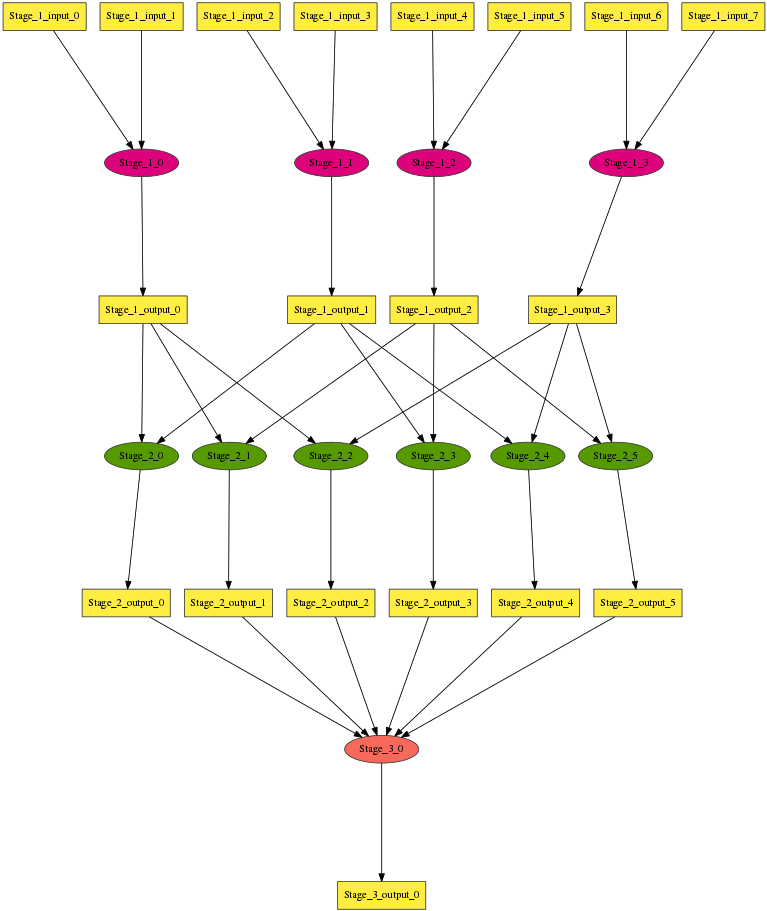
\includegraphics[width=85mm]{pictures/sample}
\caption {Task flow of the three-stage application
   \label{fig:sample}
}
\end{figure}


\subsubsection{Parameter Distribution}\label{sec:distr}
The skeleton tool implements two categories of distributions.

The first category, statistical distributions, can be used for \textbf{Task\_Length}, \textbf{Input\_File\_Size}, and \textbf{Output\_File\_Size}.

If \textbf{Task\_Length}, \textbf{Input\_File\_Size}, \textbf{Output\_File\_Size} are to be described as statistical distributions, one of the distributions and formats in Table~\ref{tb:distributions} should be used.

\begin{table}[h]
\begin{center}
\caption{Statistical Distributions}

\label{tb:distributions}
\vspace{4pt}
    \begin{scriptsize}
\begin{tabular}{|c|c|c|}
\hline
Name & Format & Example \\
\hline
\hline
uniform & [number][unit] & 5s, 1048576B\\
\hline
normal & [avg, stdev][unit] & [5, 1]s, [1048576, 1000]B\\
\hline
triangular &[avg, stdev][unit] & [5, 1]s, [1048576, 1000]B\\
\hline
lognorm & [avg, stdev][unit] & [5, 1]s, [1048576, 1000]B\\
\hline
\end{tabular}
    \end{scriptsize}
\up\up
\end{center}
\end{table}

%\begin{itemize}
%
%\item{\textbf{uniform}}: [number][unit], e.g. 5s, 1048576B
%
%\item{\textbf{normal}}: [avg, stdev][unit], e.g. [5, 1]s, [1048576, 1000]B
%
%\item{\textbf{triangular}}: [avg, stdev][unit], e.g. [5, 1]s, [1048576, 1000]B
%
%\item{\textbf{lognorm}}: [avg, stdev][unit], e.g. [5, 1]s, [1048576, 1000]B
%
%\end{itemize}


The second category, dependent distributions, can be used for \textbf{Task\_Length} and  \textbf{Output\_File\_Size}.  \textbf{Task\_Length} can be a polynomial function of \textbf{Input\_File\_Size}, and \textbf{Output\_File\_Size} can be a polynomial function of  \textbf{Task\_Length} or \textbf{Input\_File\_Size}.

The \textbf{Task\_Length} can be a polynomial function of \textbf{Input\_File\_Size} if and only if there is one input file per task. This is described as:
\begin{shortlist}
\item[]{\textbf{input}}: [coefficient, power]x, e.g. [4, 2]x
\end{shortlist}
where task length is computed as: \( \text{coefficient} * \text{filesize} ^ \text{power}\). 
Listing~\ref{lst:inputfunc} shows an example of this.

\begin{lstlisting}[caption= Task length as a function of input file size, label=lst:inputfunc, linewidth=1.0\textwidth, xleftmargin=2.5ex]
Num_Stage = 1

Stage_Name = Stage_1
    Num_Tasks = 4  
    %*\texttt{\textbf{Task\_Length = input [4, 2]x}}*)
    Input_Source = filesystem
    Input_Files_Each_Task = 1
    Tasks_Each_Input_File = 1
    Input_File_Size = normal [1048576, 1000]
    Output_Files_Each_Task = 1
    Output_File_Size = normal [1048576, 1000]
\end{lstlisting}

\subsubsection{File-Task Mapping}\label{sec:def_mapping}

As previously mentioned, mapping files between stages can be done either based on a default mapping implied by 
\textbf{Input\_Files\_Each\_Task} and \textbf{Tasks\_Each\_Input\_File}, or by an external mapping routine.

The default file-task mapping is calculated by the value of \textbf{Input\_Files\_Each\_Task} and \textbf{Tasks\_Each\_Input\_File}.
If \textbf{Tasks\_Each\_Input\_File} is 1, then \textbf{N} tasks shall have \textbf{N*Input\_Files\_Each\_Task} distinct input files, with
each task mapped to \textbf{Input\_Files\_Each\_Task} input files, such as in lines 7 and 8 in Listing~\ref{lst:sample}.
%
If \textbf{Input\_Files\_Each\_Task} is set to the number of distinct input files (the number of input files
is implicitly set to $\frac{\textbf{Input\_Files\_Each\_Task*Num\_Tasks}}{\textbf{Tasks\_Each\_Input\_File}}$, or inherited from previous stage),
and \textbf{Tasks\_Each\_Input\_File} has the same value as \textbf{Num\_tasks}, then each task in this stage maps to all input files, such as in lines 26 and 27 in Listing~\ref{lst:sample}.



External mapping option can be used to describe more complex mappings between tasks and files.
An optional parameter, \textbf{Input\_Task\_Mapping}, overrides the default file-task mapping.
Currently, this can only be set to \textbf{External}.
 External mapping requires an shell executable that outputs the file grouping to standard output, with each line in a row, and with files  delimited by white space.
Listings~\ref{lst:exmapper} and \ref{lst:excode} show an use case and a sample implementation of the external mapper, respectively.
The naming rule for the files is: Stage\_Name\_fileusage\_fileid, e.g., Stage\_1\_input\_0. The Skeleton tool only checks the naming correctness of the file names produced by the external mapper: the file names have to start with the stage name, and output files of other stages have to exist before they are mapped to tasks.

\begin{lstlisting}[caption=Use case of external mapper, label=lst:exmapper, linewidth=1.0\textwidth, xleftmargin=2.5ex]
Num_Stage = 1

Stage_Name = Stage_1
    Num_Tasks = 4  
    Task_Length = normal [10, 1]s
    Input_Source = filesystem
    Input_Files_Each_Task = 2
    Tasks_Each_Input_File = 1
    Input_File_Size = normal [1048576, 1000]M 
    %*\texttt{\textbf{Input\_Task\_Mapping = External external.sh}}*)
    Output_Files_Each_Task = 1
    Output_File_Size = normal [1048576, 1000]M
\end{lstlisting}

\begin{lstlisting}[language=Bash, caption=Sample code of external mapper, label=lst:excode, linewidth=1.0\textwidth, xleftmargin=2.5ex]
#!/bin/bash

echo Stage_1_input_0 Stage_1_input_4 
echo Stage_1_input_3 Stage_1_input_5
echo Stage_1_input_1 Stage_1_input_6
echo Stage_1_input_2 Stage_1_input_7
\end{lstlisting}

\section{Evaluation} \label{sec:eval}

To compare the performance of the Skeleton application and the real application, we use a 6x6 degree image mosaic
example from Montage~\cite{montage1} and the first 256 queries of the NRxNR test of BLAST~\cite{ParallelBlast} on 64 IBM BG/P processors. 
%\note{and ... of BLAST on ...}
The tasks are launched with AMFS~\cite{AMFS2013} and the input
and output files are read and written from/to the GPFS shared filesystem. Figure~\ref{fig:Montage} shows the data flow patterns between Montage
stages.

\begin{figure}[h]
\begin{center}
    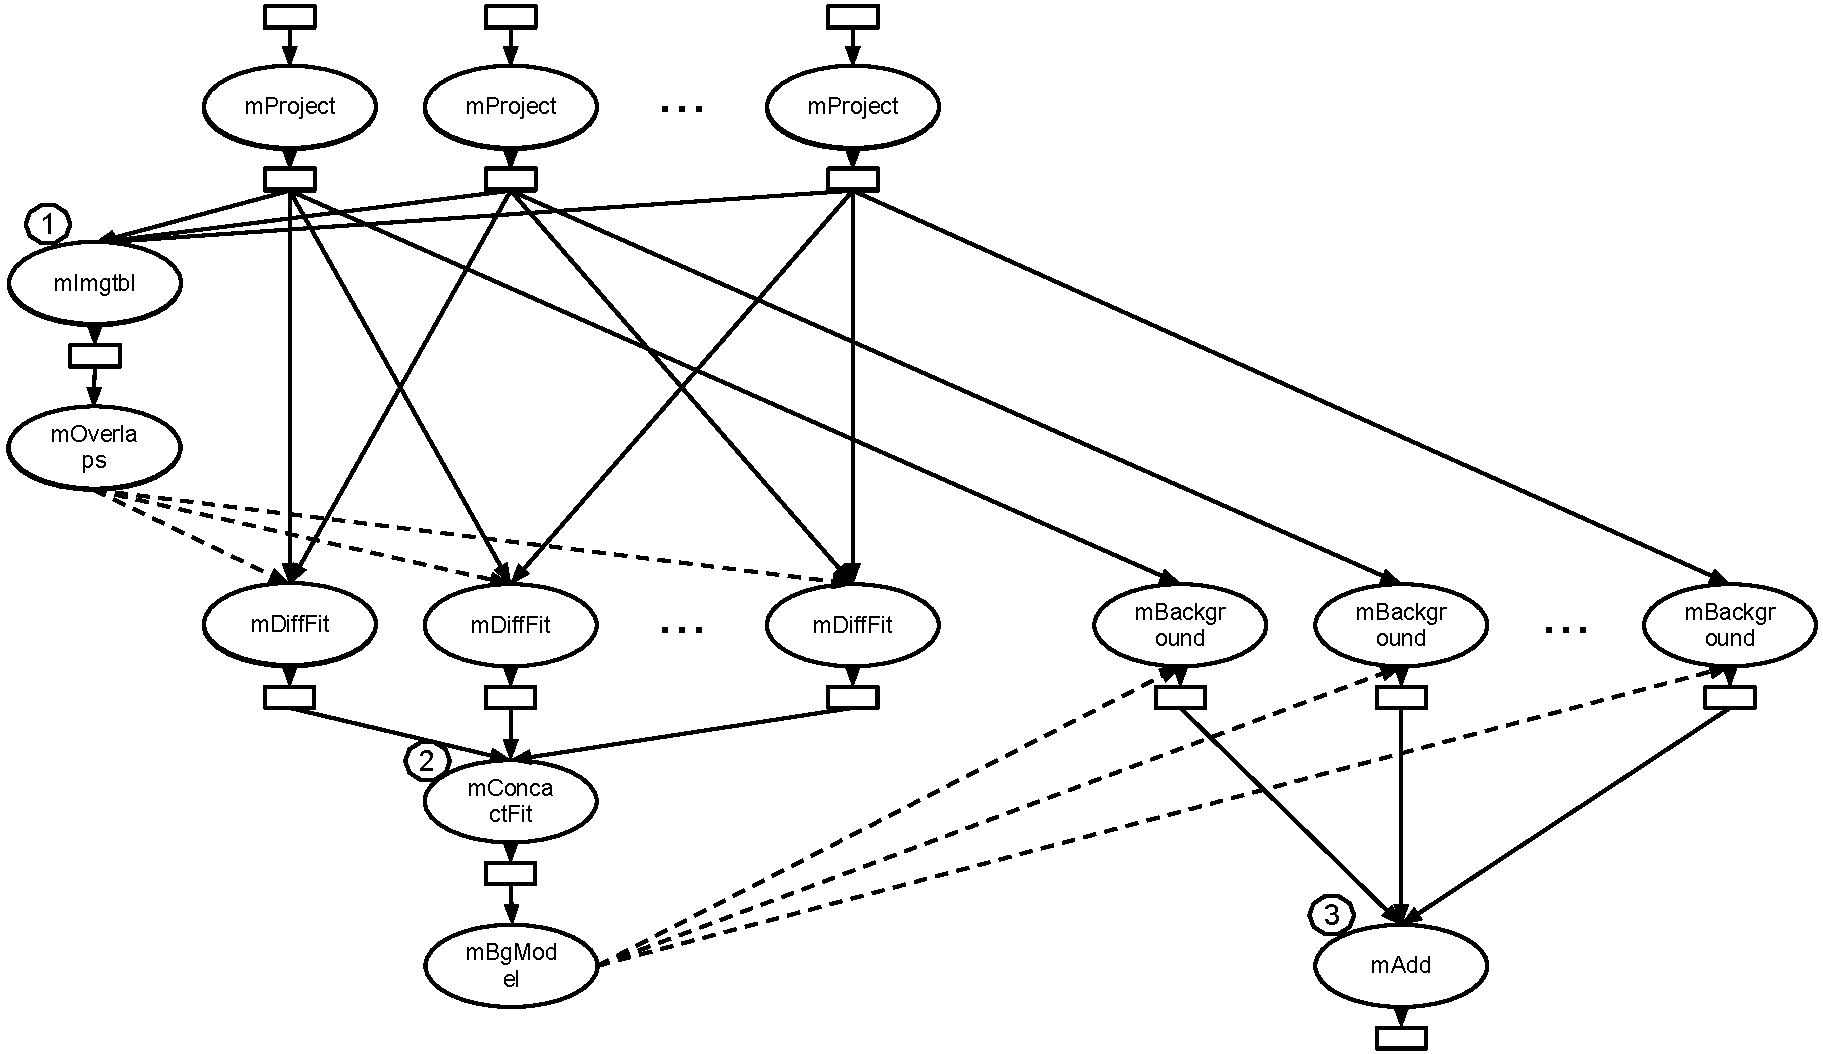
\includegraphics[width=85mm]{pictures/Montage}
\caption {Montage dataflow. Ovals represent tasks and boxes files. Solid lines show file transfers, dashed lines show additional control flow dependencies.
    \label{fig:Montage}
}
\end{center}
\end{figure}

%\subsection{Montage}
\begin{table*}[t]
\begin{center}
    \caption{Number of tasks, inputs, and outputs, and input and output size, for each Montage stage}
    \begin{scriptsize}
    \begin{tabular}{ | p{1.6cm} | p{1cm} | p{1cm} | p{1.2cm} | p{1cm} | p{1.25cm} | p{2cm} | p{1.5cm} | p{1.5cm} |}
    \hline
    Stage & \# Tasks & \# Inputs & \# Outputs & In (MB) & Out (MB) & Measured Time Avg (sec) & Measured Time Stdev & Skeleton Task Length\\ \hline \hline
	mProject & 1319 & 1319 & 2594 & 2800 & 10400 & 11.1 & 2.5 & 12\\ \hline
	mImgtbl & 1 & 1297 & 1 & 5200 & 0.8 & N/A & 0 & 16\\ \hline
	mOverlaps & 1 & 1 & 1 & 0.8 & 0.4 & 9 & 0 & 9\\ \hline
	mDiffFit &  3883 & 7766 & 7766 & 31000 & 487 & 1.7 & 0.6 & 2\\ \hline
	mConcatFit & 1 & 3883 & 1 & 1.1 & 4.3 & 14 & 0 & 14\\ \hline
	mBgModel & 1 & 2 & 1 & 4.5 & 0.07 & 283.1 & 0 & 284 \\ \hline
	mBackground & 1297 & 1297 & 1297 & 5200 & 5200 & 0.4 & 0.08 & 1\\ \hline
	mAdd  & 1 & 1297 & 1 & 5200 & 7400 & N/A & 0 & 519\\ \hline

    \end{tabular}
    \end{scriptsize}
    \label{tb:stats}
    \up
\end{center}   
\end{table*}

Table~\ref{tb:stats} shows basic statistics for each Montage stage. Measured Time Avg shows the average time-to-solution of all tasks in each stage.  The Skeleton Task Length column  shows the exact task length we set in the Skeleton, determined as follows:  
%This task length is measured by reading/writing files on RAM disk, which eliminates the I/O overhead of the shared file system. 
%\zhaonote{explaining how to estimate task length for each stage}
For the mProjectPP, mOverlaps, mDiffFit, mConcatFit, mBgModel, and mBackground stages,  we place the input/output files on RAM disk then round 
the average time-to-solution up to the nearest integer as the task length. 
For stages of mImgtbl and mAdd, the input size exceeds the RAM disk size on a compute node,
so we cannot execute the tasks with the data on RAM disk. Based on observation and validation, we see that the
task's time-to-solution is proportional to the number of input files when the file number is small (10-30), so we project the
time-to-solution with the full input data set based on
the measured time-to-solution on a smaller data set. 


\begin{table*}[]
\begin{center}
    \caption{Time-To-Solution Comparison of Skeleton Montage and Real Montage (seconds)}
    \begin{scriptsize}
    \begin{tabular}{ | p{1cm} | p{1cm} | p{1cm} | p{1.2cm} | p{1cm} | p{1.4cm} | p{1.2cm} | p{1.8cm} | p{1cm} | p{1cm} |}
    \hline
	& mProject & mImgtbl & mOverlaps & mDiffFit & mConcatFit & mBgModel & mBackground & mAdd & Total\\ \hline \hline
	Montage & 290.4 & 139.7 & 10.2 & 359.2 & 64.6 & 283.3 & 102.6 &  793.4 & 2040.6\\ \hline
	Skeleton & 283.4 & 124.3 & 10.5 & 313.5 & 67.0 & 283.2 & 98.2 &  807.6 & 1987.6\\ \hline
	Error & -2.4\% & -11.1\% & 2.9\% & -12.7\% & 3.9\% & -0.04\% & -4.3\% & 1.8\% & -2.6\%\\ \hline
    \end{tabular}
    \end{scriptsize}
    \label{tb:results}
    \up\up
\end{center}   
\end{table*}

In the Skeleton configuration for the stages where there are a large number of input/output files of the same size, (mProject, mImgtbl, mDiffFit, mBackground and mAdd), 
we specify that all files for a stage are that size. 
%\katznote{why do we do this?  are they all the same size?  or this an average and we then will set them all to the average, as we do for mConcatFit too?} 
%\zhaonote{for each stage of mProject, mImgtbl, mDiffFit, mBackground, and mAdd, the input/output files are the same size. Input of mProject: 2.1 MB each, Output: 4.2MBx2. mImgtbl input: 4.2MBx1297. mDiffFit input: 4.2MBx7766. mBackground input: 4.2MBx1297. mAdd input: 4.2MBx1297. The only exception is the input of mConcatFit which is also the output of mDiffFit, the file sizes are not so close to each other, so we use the average file size to specify this group of files.}
%This is true for mProject, mImgtbl, mDiffFit, mBackground and mAdd.
For mConcatFit, the 
input file sizes vary from 157 bytes to 292 bytes. To simplify the the Skeleton specification, we set all input files of mConcatFit 
(the output of mDiffFit) to the average file size of 200 bytes.
%\katznote{what's the point of this paragraph?  The first part is how we run the real app, the second says we can't run the skeleton this way?  but why not?  And, why does this paragraph go here between how we set skeleton parameters in the previous paragraph and how we set them in the next paragraph?} 
%\zhaonote{this also refers to the point I made in long future work: if we run a task of mProject with the files on GPFS, the process opens, reads, writes, and closes the file on GPFS. The computation and I/O can be actually interleaved. The sequence can be random: read-compute-read-compute-write-read-compute-read-write-compute. But with the current implementation of Skeleton, we simplify the computation and I/O as a read-compute-write model. If we run the skeleton and real app on GPFS, the skeleton should be a lot faster than the real app, just as what we did in the SC12 paper comparing Montage performance with files directly on GPFS and staging files to RAM}
%\zhaonote{this paragraph explains how we measure the real application time, so it follows how we specify skeleton configurations. Shall we move it before skeleton configuration?}
Note that for both the real Montage application and the Skeleton, we use a staging approach to execute the task: we first copy the input files
from GPFS to RAM disk, execute the task, write the output files to RAM disk, then copy the output files back to GPFS. 
%This is the same as what the Skeleton version of Montage does.
%This is due to one limitation of the current Skeleton implementation. Skeleton-produced tasks can not mimic the interleaved computation/IO
%behavior exactly as a real task. We over simplified this process as read-compute-write model. We will improve this feature later.

Table~\ref{tb:results} compares performance of the Montage Skeleton with the real Montage application on 64
IBM BG/P quad-core processors with GPFS as the shared filesystem. For each data point, we measured the performance three
times and show the average value. In total, the Skeleton Montage runs in 2.6\% less time the real Montage application.

Among the eight stages, mProject, mDiffFit, and mBackground are those with parallel execution. The measured error is -2.4\%,
 -12.7\% and 1.8\% respectively. The significant error of mDiffFit is due to the time-to-solution distribution of all tasks: a distribution
with an average of 1.7 seconds and a standard deviation of 0.6. The ratio between standard deviation and average is 35.4\%, while the ratio
for mProject and mBackground is 22.5\% and 20.0\% respectively. This higher ratio implies a higher variability of mDiffFIt tasks, thus using
average time-to-solution for all tasks should result worse precision than the other two stages. We believe this gap can be improve by using Skeleton's
statistical distribution functionality. 
%\katznote{why didn't we do this then?}\zhaonote{this is an implementation limitation, I should have done
%this, but haven't. The current implementation of Skeleton only accepts statistical distributions as "dist [avg, stdev]unit", and the format that can
%be accepted is string [int, int]char, which limits the setting to be integer. We need to fix this to let users set float numbers, it is in the TODO list. }

mOverlaps, mConcatFit, and mBgModel each have a single task, and the input/output fit in a compute node's RAM disk. The Skeleton
versions have errors of 2.9\%, 3.9\% and -0.04\%. 
mImgtbl and mAdd are each a single task with 1297 input files, whose size exceeds a single node's RAM disk size. 
With the projected task length, the errors of the two stages are
-11.1\% and 1.8\%. We can tell that mImgtbl's time-to-solution grows more than linearly with the number of input files as the variable, while
mAdd's time-to-solution grows close to linearly. 
%\katznote{how could we fix the prediction for mImgtbl?}\zhaonote{I don't have a solution yet,
%ideally, we could run it on the same CPU but with a larger RAM disk.}

%\subsection{BLAST}
%\textcolor{red}{To the reviewers: In the camera-ready version of this paper, we will use the Skeleton configuration option of distribution functions to more closely approximate task runtimes and show  improved accuracy. We also plan to add results for a second application, BLAST.  We apologize for not having done this work in time for this submission.}

For BLAST, we run the first 256 queries from the NRxNR test case on 64 BG/P compute nodes. We set up the task length as uniform for the formatdb and blastp stages. The task lengths of the merge stage vary from one second to 14 seconds, so we use the actual task length for these 16 skeleton tasks. 
%\katznote{what does this mean?}
%\zhaonote{The merge stage has 16 tasks, their running times are 1, 1, 1, 2, 3, 3, 3, 3, 4, 4, 4, 5, 6, 12, 13, 14 seconds. I tried to use the average 4 seconds as running time, then the Skeleton runs to much shorter than real BLAST. I also thought about using distributions, but there was not a clear pattern what distribution this was. So I just used these running times for the tasks. And the above sentence tells what I did.}
The input file sizes of formatdb tasks are uniform, but the outputs are not. Each formatdb task has three output files, their sizes are 56 MB, 16MB, and 1MB respectively. Due to the limitation of the present Skeleton implementation, we define the synthetic output files as 3, with uniform size of 21 MB.
Table~\ref{tb:blast-stats} shows some basic statistics of BLAST stages and Table~\ref{tb:blast-results} shows the measured performance and the comparison between the Skeleton BLAST and real BLAST. 

The formatdb stage's error is 7.2\%. One possible reason is that the real formatdb task has $\sim$500,000 small writes, each with hundreds of bytes, while our Skeleton synthetic application's writes has a much larger buffer. The 8.0\% error of blastp stage could be due to the uniform task length distribution, as the real distribution ranges from 80s to 160s.
The predicted merge time-to-solution is low because of the per sequence reads of the input files, which are each hundreds of bytes, while the Skeleton merge has a single large read.  

\begin{table*}[t]
\begin{center}
    \caption{Number of tasks, inputs, and outputs, and input and output size, for each BLAST stage}
    \begin{scriptsize}
    \begin{tabular}{ | p{1.6cm} | p{1cm} | p{1cm} | p{1.2cm} | p{1cm} | p{1.25cm} | p{2cm} | p{1.5cm} | p{1.5cm} |}
    \hline
    Stage & \# Tasks & \# Inputs & \# Outputs & In (MB) & Out (MB) & Measured Time Avg (sec) & Measured Time Stdev & Skeleton Task Length\\ \hline \hline
	formatdb & 64 & 64 & 192 & 3800 & 4400 & 41.9 & 0.1 & 42\\ \hline
	blastp & 1024 & 4096 & 1024 & 70402 & 966 & 109.2 & 14.9 & 110\\ \hline
	merge & 16 & 1024 & 16 & 966 & 867 & 4.4 & 4.1 & real length\\ \hline
    \end{tabular}
    \end{scriptsize}
    \label{tb:blast-stats}
    \up
\end{center}   
\end{table*}

 
\section{Related Work}  \label{sec:related}
Skel~\cite{Skel} uses a similar idea to understand the I/O performance of parallel applications on supercomputers. Users can extract 
the I/O behavior from an application, then produce a skeletal application that mimics the I/O operations and pattern by specifying
a Skel configuration file. The produced skeletal application can run on ADIOS~\cite{ADIOS}. WGL~\cite{WGL} lets users generate a Swift script for a
workflow application by describing the data flow patterns between stages.


\section{Conclusions and Future Work} \label{sec:end}

We have shown the Skeleton tool can produce synthetic distributed applications that correctly capture important distributed properties of real applications but are much simpler to define and use.
The Skeleton tool currently can generate applications that represent bag-of-tasks, MapReduce, and multi-stage workflows.
Skeleton applications can be run with mainstream workflow frameworks and systems: Shell, Pegasus, and Swift.
The execution comparison between the the initial Skeleton Montage and BLAST and the real Montage and BLAST on 64 BG/P processors shows an acceptable runtime difference  of 2.6\% and 8.0\%, and for each individual
stage, the difference ranges from 0.04\% to 12.7\%, with six out of eleven stages within 5\%.  These can be improved by more carefully configuring the Skeleton.

In the near future, we will open source the Skeleton code, and invite users and contributors from a wider community to try it and expand it.
%
Our longer term plan includes: 
\begin{shortlist}
\item {} Use application trace data to produce synthetic applications ideally purely from the trace data but initially from a combination of trace data and user guidance.
\item {} Determine a way to represent the computational work in a task that when combined with a particular platform can give an accurate runtime for that task.
\item {} Support tasks with interleaved computation and I/O, rather than just read-compute-write.
\item {} Support tasks that are not generic single core tasks, such as those that internally include OpenMP or MPI, or those that should be bound to specific hardware, e.g., GPUs.
\item {} Support concurrent tasks that need to run at the same time to exchange information.
\item {} Support iterations in Skeleton configuration model.
\item {} Investigate an accurate task-file mapping specification that supports cases other than 1-1 and n-1 that requires less user programming. 
\end{shortlist}

\begin{table}[t]
\begin{center}
    \caption{Time-To-Solution Comparison of Skeleton BLAST and Real BLAST (seconds)}
    \begin{scriptsize}
    \begin{tabular}{ | p{1cm} | p{1cm} | p{1cm} | p{1.2cm} | p{1cm} | }
    \hline
	& formatdb & blastp & merge & Total \\ \hline \hline
	BLAST & 82.1 & 1996.3 & 35.9 & 2114.3 \\ \hline
	Skeleton & 76.2 & 1835.9& 34.0 & 1946.1 \\ \hline
	Error & 7.2\% & 8.0\% & 2.9\% & 8.0\% \\ \hline
    \end{tabular}
    \end{scriptsize}
    \label{tb:blast-results}
    \up
\end{center}   
\end{table}

\section*{Acknowledgments}

This work was supported in part by the U.S. Department of Energy 
under the ASCR award DE-SC0008617 (the AIMES project).
It has benefited from discussions with Shantenu Jha, Andre Merzky, Matteo Turilli, Jon Weissman, and Lavanya Ramakrishnan.
Computing resources were provided by the
Argonne Leadership Computing Facility. Work by Katz was supported by 
the National Science Foundation while working at the Foundation.  Any 
opinion, finding, and conclusions or recommendations expressed in this
 material are those of the author(s) and do not necessarily reflect 
 the views of the National Science Foundation.
 
\bibliographystyle{abbrv}
\bibliography{Skeleton}

% that's all folks
\end{document}
